\documentclass[10pt,a4paper]{proc}

\usepackage{graphicx}

\begin{document}
\title{Home Assignement}
\author{Lorenzo Corneo (890225-1290) \\ Antonios Kouzoupis (890121-8837)\\
	\{corneo, antkou\}@kth.se}
\date{\today}
\maketitle

\section{System specification}
Before showing the evaluation on the experimentations, it is necessary to explain briefly how we implemented the SWIM protocol and how we solved the problem of the NATs. 

The aim of this report is not a full description of the system, but some knowledge is necessary to better understand the results we got in the evaluation phase.

\subsection{SWIM}
In this section it is explained what we did different than what was required from the specification of the assignment.

To begin with, it is required to piggyback information only during the ping but we strictly followed the SWIM paper and the propagation of such information happens also during the ping phase. In our opinion, this accelerate the convergence of the overlay as the changes are spread faster.

Then, when a pong is received, the peer selects up to \texttt{PIGGYBACK\_SIZE} peers from the membership list, accordingly to its size, which have infection time smaller than the upper-bound. If the pong it is not received, the node sends an indirect-ping request to N random selected alive nodes.

Finally, as long as we believe that the random peer selection for the ping operation may not be optimal, we decided to implement a round-robin selection as suggested by the paper. A counter of pings is maintained and the selection happens between those peers with the lowest value. When a new peer joins the membership list, its counter is set to the minimum value (and not to zero) so that it will not be pinged many time sequently until it reaches the actual minimum.

\subsection{SWIM through NATs}

This section explains how we overcame the problem and how we propagate through the overlay changes in the parents list of the peers behind a NAT.

Peers behind NAT are not directly reachable so they must have relay peers which are open (they don't have NAT) and forward their traffic (in and out) through the network. The SWIM component propagates information also of the parents of peers behind NAT, so that other nodes know how to contact them. The NatComponent constantly sends heartbeats to the parents nodes in order to check whether they are still alive.

When the NatComponent discovers a parent is dead it gets new nodes from the CroupierComponent. The Croupier component returns a set of nodes that contains also dead nodes. For this reason, when the NatComponent receives this set, it queries the SwimComponent to check whether the nodes of the set are alive or dead. Up to an upper-bound of the alive nodes are set to be new parents for that node. Of course, the NatComponent can check itself whether the new candidate parents are alive, but this would add complexity to the component and, most of all, the SwimComponent already provides this service.

\section{Evaluation}

The assignment asks to retrieve the convergence time for different configuration, considering infection time, piggybacked information, number of peers and number of peers behind a NAT.

The SWIM protocol is highly configurable and, in particular, the most important parameters to configure are the infection time and the size of the piggybacked information. The authors of the paper suggest the infection time should be $\lambda logn$

This is not all, to guarantee the convergence in our experimentation we also varied the number of peers behind the NAT. For instance, if the number of those peers is too high the overlay will not converge.

\subsection{Considerations}

We were not completely sure about the validity of those results because when we ran again the experimentations we got different results. Nonetheless, the theoretical studies done on SWIM made us able to know about the existence of an optimal configuration of the parameters. 

After a deep analysis, we understood the gap between simulations on the same scenario was because we took timing in real-time. The Kompics framework utilises simulation time so that our results may be affected by the actual load of the CPU.

To solve this issue, we decided to implement a timer (with period 100ms) inside the AggregatorComponent which increments a variable accordingly to the time used by Kompics. Still, we don't obtain the real time but at least we get a consistent time.

Additionally, we considered also the fact that the most of the system is deterministic, because we seed the random number generator always with the same value. On the contrary, the CroupierComponent is not deterministic as it provides different samples in every execution. Thus, some set of results might not match with the expected theoretical ones.

\subsection{Experimentation results}

In the following experimentations we focused mainly in finding boundary cases (between non convergence and convergence) and studying the variation of the performance varying both the infection time and the piggyback size.

We are seeking for \emph{convergence} and we find two types of it, depending on the scenario. Convergence may mean either, in case of only alive nodes, the time used for the whole network to know every peer or, in case of dead nodes, the time elapsed to propagate the failures to all the alive nodes.

In Figure \ref{allAliveNoKill} we present the results of a simulation with 300 peers, 250 of these were open whilst 50 were behind a NAT. We must notice that the minimum configuration to get convergence is ($\lambda=9$, ps\footnote{Piggyback size.}=60). We observed the lowest convergence time (52,926ms) for the configuration ($\lambda=10$, ps=70). For lower values of $\lambda$ or ps, the system took more time to converge because of the low propagation of the piggybacked information. The same effect appears also for too big values, this made us aware that there is an optimal configuration of these parameters.

\begin{figure}
\centering
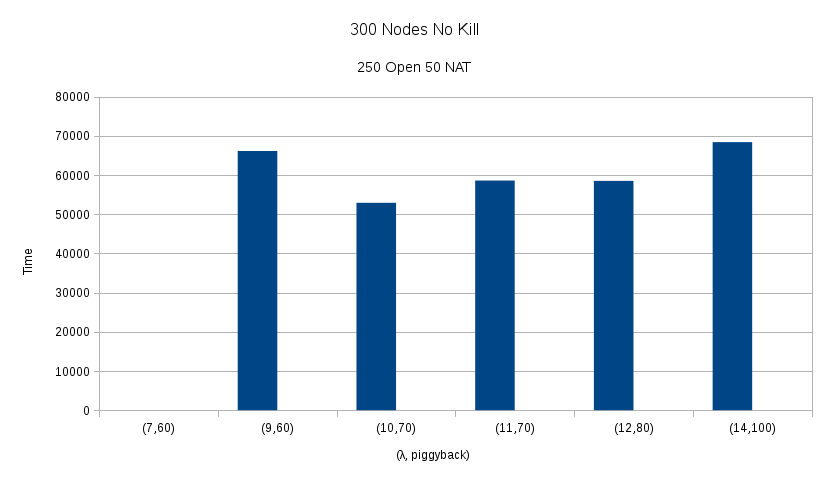
\includegraphics[scale=0.35]{metrics/allAliveNoKill.png}
\caption{300 nodes without killing.}
\label{allAliveNoKill}
\end{figure}

In Figure \ref{allAliveIndirect} we use the same setting of the previous scenario but we delete some of the connection between the peers of the overlay. As expected, nothing change but the performance. In fact, because of the indirect ping nodes take more time to reach the target of the ping.

\begin{figure}
\centering
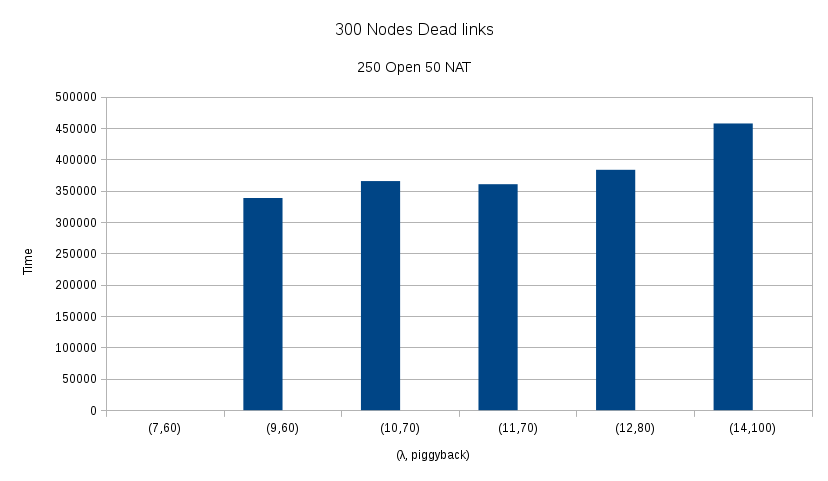
\includegraphics[scale=0.35]{metrics/allAliveIndirect.png}
\caption{300 nodes with indirect ping.}
\label{allAliveIndirect}
\end{figure}

In Figure \ref{allAliveFixedLamda} we measure the variation of the convergence time keeping a fixed value for $\lambda$ and varying the piggyback size. What we observed is that for big values of piggyback size we have better convergence time as the information are spread faster through the network.

\begin{figure}
\centering
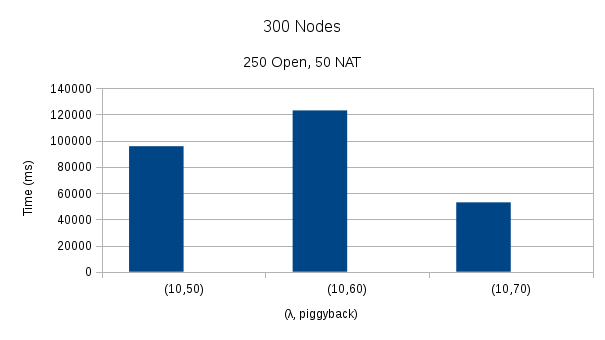
\includegraphics[scale=0.5]{metrics/allAliveFixedLamda.png}
\caption{300 nodes $\lambda=10$.}
\label{allAliveFixedLamda}
\end{figure}

The next experiment (Figure \ref{kill15Open}) includes 130 nodes. 100 of them are open and 30 are behind NATs. After 5 seconds we kill 15 open nodes and 8 NATed nodes. The results show two good convergence time and one much higher ($\lambda=22$, ps=40), this effect because the infection time is not well dimensioned according to the piggyback size and viceversa. This experiment is quite hard to converge because it might happen that parents of NATed nodes die consecutively.

\begin{figure}
\centering
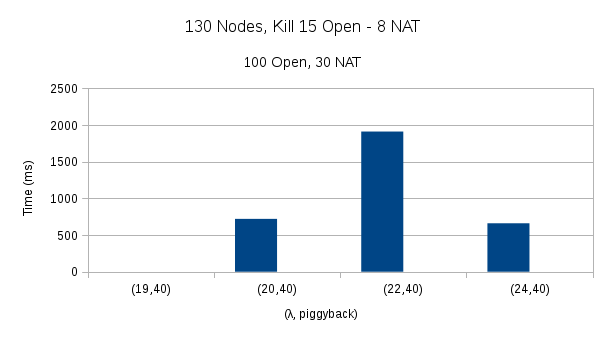
\includegraphics[scale=0.5]{metrics/kill15Open.png}
\caption{130 nodes with 23 kills.}
\label{kill15Open}
\end{figure}

Figure \ref{kill15OpenFixed} we execute the same experiment previously discussed but we keep a constant value $\lambda=24$. In this case the results are very good as we can observe that the convergence time is inversely proportional to the piggyback size. To put it in other words, the performance is better when we piggyback more information at the same time.

\begin{figure}
\centering
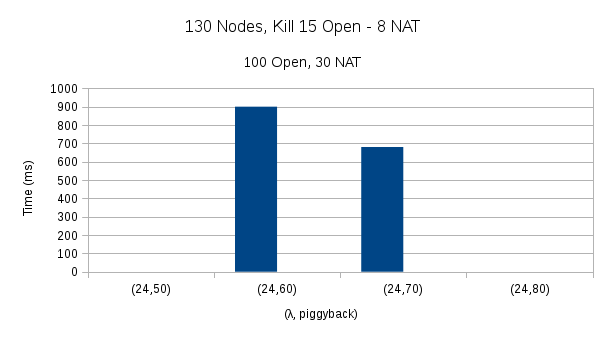
\includegraphics[scale=0.5]{metrics/kill15OpenFixedLamda.png}
\caption{130 nodes with 23 kills and $\lambda=24$.}
\label{kill15OpenFixed}
\end{figure}

The last experiment we report here (Figure \ref{kill5Open}) we have 80 nodes (60 open and 20 NATed). After 3 seconds we kill 5 open peers and 12 NATed peers, for a total of 17. Here we keep a fixed value for ps=40 and we vary $\lambda$. We observe a strange climax in the convergence time nearly 100000ms as we expected a value lower then for $\lambda=6$. Except for this value, the global trend of the performance matches the expected results.

\begin{figure}
\centering
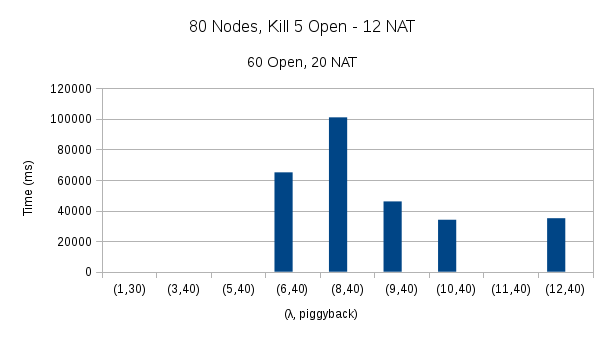
\includegraphics[scale=0.5]{metrics/kill5Open.png}
\caption{80 nodes with 17 kills.}
\label{kill5Open}
\end{figure}

\section{Conclusion}

The results we got are very meaningful because they made us understand that a underestimation of the parameters leads to the non convergence whilst an overestimation leads to a degradation of the convergence time.

Additional negative effects can be obtained, for example, when too many open nodes are killed at the same time so that it is impossible for the nodes behind a NAT to made them reachable by other peers.

To conclude, it is interesting, for future work, to implement a partial view rather than a global one that, of course, may saturate the memory of the machine.

\end{document}